 \documentclass[12pt]{spieman}  % 12pt font required by SPIE;
%\documentclass[a4paper,12pt]{spieman}  % use this instead for A4 paper
\include{moritz}
\usepackage{amsmath,amsfonts,amssymb}
\usepackage{graphicx}
\usepackage{setspace}
\usepackage{tocloft}
\usepackage{gensymb}
\usepackage{lineno}
\linenumbers

\title{A concept for a critical-angle transmission grating spectrometer for the AXIS probe}
\author[a]{Hans M. G\"unther}
\author[a]{Other authors here.... including}
\author[a,b]{Ralf K. Heilmann}
\affil[a]{MIT Kavli Institute for Astrophysics and Space Research, Massachusetts Institute of Technology, Cambridge, MA 02139, USA}
\affil[b]{Space Nanotechnology Laboratory, Massachusetts Institute of Technology, Cambridge, MA 02139, USA}

\renewcommand{\cftdotsep}{\cftnodots}
\cftpagenumbersoff{figure}
\cftpagenumbersoff{table}
\begin{document}
\maketitle

\begin{abstract}
AXIS is a probe-class mission study in response to the 2020 Astrophysics Decadal Survey, which recommended two competed probe-class missions and specifically calls out an X-ray probe with high spatial and spectral resolution. AXIS will feature large collecting area with a point-spread-function (PSF) of order 1-2 arcsec. We describe a possible X-ray grating spectrometer (XGS) that could be added to AXIS with minimal design changes to the telescope itself at a cost of just a few percent of the total mission budget. The XGS would be based on critical-angle transmission (CAT) gratings, developed for Arcus and Lynx. Using detailed ray-tracing, we investigate several options for sub-aperturing which provide a trade-off between effective area and spectral resolving power. Covering about 1/3 of the full aperture with gratings, we find a  high spectral resolving power $\lambda/\Delta\lambda \approx 5000$ and effective area around 500~cm$^2$ in the soft x-ray band (1.5-3.5 nm). CAT gratings are mostly transparent at high energies, and thus hard x-rays can still be used for simultaneous imaging spectroscopy. We study different grating sizes and other enhancements, but even in the basic configuration an XGS can be added to AXIS to provide the high-resolution spectral capabilities that the  Astrophysics Decadal Survey calls for. Our ray-tracing shows that this concept is mature and can be added to AXIS with minimal impact on other instruments. We discuss one exemplary science case that would be enabled by the XGS.

\end{abstract}

\keywords{ray-tracing, X-ray optics, critical-angle transmission grating, AXIS, Rowland torus, grating spectroscopy}

% Include email contact information for corresponding author
{\noindent \footnotesize\textbf{*}Hans M. G\"unther,  \linkable{hgunther@mit.edu} }

% Activate this before submission
%\begin{spacing}{2}   % use double spacing for rest of manuscript
% But for display on the screen in overleaf it is much easier to look at single spaced
% text because it does not require constant scrolling
\begin{spacing}{1}



\section{Introduction}
\label{sect:introduction}
The NASA 2020 Decadal Survey ``Pathways to Discovery in Astronomy and Astrophysics for the 2020s''\cite{2021pdaa.book.....N} recommends the implementation of a Probe-class line of missions with the first mission to the selected from proposals for Far-Infrared or X-ray missions. Probe-class missions are located between NASA's medium explorer (MIDEX) programs and multi-billion dollar flagship missions. The Advanced X-ray Imaging Satellite (AXIS) was proposed as a white paper \cite{2019BAAS...51g.107M} to the decadal survey and the concept has been continuously developed since. AXIS would would use a Si meta-shell approach to nest a large number of precisely formed Si mirrors to achieve a high effective area about two orders of magnitude better than Chandra, while maintaining a Point-Spread-Function (PSF) of order 1-2 arcsec over a larger field of view. Mirrors and detectors are optimized to function over a similar range of energies as Chandra and XMM-Newton do today, from about 0.3 to 10~keV.

With these characteristics, AXIS will deliver much sharper images than the planned Athena mission\cite{doi:10.1117/12.2188988,doi:10.1117/12.2057347}. AXIS would target a few specific science cases, such as galaxy evolution and feedback, the growth of black holes, and active galactic nuclii (AGN) in the high-redshift universe, but importantly function as a proposal-driven observatory that provides unique capabilities to a large range of science questions.

The basic optical setup of AXIS includes just the mirror and an imaging spectrometer such as a CCD array at the focal plane. The CCD (or similar device) will provide low-resolution spectroscopic capabilities, but particularly in the soft-X-ray band the best CCD energy resolution is only of order 70~eV or so. In this work, we show that a grating spectrometer can outperform a CCD in soft X-rays by more than two orders of magnitude in terms of resolving power and thus enable fundamentally new science investigations that resolve emission or absorption lines profiles from stars, black holes, and galaxies, or detect weak absorption lines from e.g.\ the warm-hot intergalactic medium super-imposed on background continuum sources.

Currently, the AXIS team does not plan to add a grating spectrometer, but we present a design based on critical-angle transmission (CAT) gratings, which can be mounted behind the mirror, either permanently or on a mechanism that folds in and out as with the highly successful Chandra High and Low Energy Transmission Gratings (HETG and LETG). CAT gratings are blazed and refract most light to just one side, where additional CCDs would be located to observe the diffracted photons.

CAT gratings\cite{Heilmann:11,doi:10.1117/12.2188525} are one of the enabling technologies for the Arcus x-ray grating spectrometer Explorer mission\cite{doi:10.1117/12.2272818}.  Arcus is designed for $R > 3500$ with $A_\mathrm{eff}$ up to $350\;\mathrm{cm}^2$ in the band between 1.2 and 5.0 nm wavelength. CAT gratings were also selected for the design reference mission for an XGS on Lynx\cite{10.1117/1.JATIS.5.2.021003}, one of the four missions concepts studied in detail before the 2020 Decadal survey\cite{10.1117/1.JATIS.5.2.021001}.

We have performed extensive ray-trace studies for both Arcus\cite{doi:10.1117/12.2273011,guntherarcus} and Lynx/XGS\cite{10.1117/1.JATIS.5.2.021003}. In particular the Lynx/XGS is quite similar to the proposed XGS for AXIS that we describe here and we refer the reader to Ref~\citenum{10.1117/1.JATIS.5.2.021003} for aspects of the design and alignment tolerances not fully covered in this article.


\section{Spectrometer design}
\label{sect:input}
The heart of a spectrometer is a collection of diffraction gratings. These will be positioned in the converging beam downstream of the mirrors. Since the resolving power $R$ increases with the distance of the dispersed signal from the focal point of the mirror, it is beneficial to mount them in a structure closely behind the end of the mirrors.

\subsection{Assumptions on the mirror}
\label{sect:PSF}
The mirror for AXIS is planned to be made from a number of Silicon Meta-shells that are made from a number of independently manufactured plates\cite{10.1117/1.JATIS.5.2.021012}. Those plates are mounted in a stack that covers some range in angle and radius and is surrounded by a support structure to hold individual plates in place. The details and dimensions of these support structure will be refined as the AXIS concept matures. In our simulations, we thus do not track all details, but instead approximate the area covered by the mirror as a series of just a few concentric rings that represent the planned radius of the meta-shell modules. All finer structures (individual plates, the angular distribution of the support structures) are treated in a statistical way: We perform a ray-trace using our code for the simplified mirrors (Iridium coated) and optical and UV blocking filters and imaging detectors. We determine the effective area that our simulations gives, which is 11500~cm$^2$. The AXIS white paper\cite{2019BAAS...51g.107M} claims an effective area of 7000~cm$^2$, so we determine a scale factor of 0.61; one minus this number can be thought of as the fraction of the geometric area of a module that is not actively concentrating light, e.g.\ because it hits the 0.5 mm thick "side" of a Si shell or because it hits some part of the mirror support structure.

In that sense, all other simulations are scaled to a zero-order effective area of 7000 cm$^2$ at 1 keV. If that area goes up or down, the effective area for the dispersed spectra scales the same way.


The mirror is simplified a perfect lens in a single plane. This simplification would give a PSF with infinitesimal width. We thus add scatter in the plane of reflection and perpendicular (``out of plane'') to the plane of reflection. If the PSF is dominated by figure errors of the mirror surface, the in-plane scatter would be much larger than the out-of-plane scatter. If, instead, it is dominated by alignment errors of Si-plates in a meta-shell module or between modules, both contributions might be similar. In most of our simulations, we assume that both contribute, with in-plane scatter just twice as large as out-of-plane scatter. A single, narrow piece of Si-mirror would give an elliptical PSF, but not that combining the PSFs of all meta-shell modules still gives a round PSF in the focal plane.
However, we also run one scenario where in-plane and out-of-plane scatter are the same and thus the PSF of a single, narrow piece of the mirror would already be round (we call this scenario ``round PSF'' referring to the PSF per meta-shell module)
To be conservative, we set up the simulations such that the total observed PSF combined from all meta-shell modules has a half-power diameter (HPD) of 1 arcsec, a factor of two worse than in the AXIS white paper \cite{2019BAAS...51g.107M}.
We do not consider diffraction from the aperture size of the individual mirror shells, because we estimate it to be small compared to the total mirror PSF\cite{Chalifoux,Raimondi}.


\subsection{CAT gratings}

\label{sect:CAT}
Critical-angle transmission (CAT) gratings have been under development for almost two decades \cite{doi:10.1116/1.2779048,doi:10.1117/12.739941,doi:10.1116/1.2968613,doi:10.1116/1.3507427,doi:10.1116/1.4755815,doi:10.1117/12.2024357,doi:10.1116/1.4820901,doi:10.1116/1.4966595}.
Using processes compatible with mass-manufacturing, they are patterned on silicon-on-insulator (SOI) wafers and etched \cite{Heilmann:11,doi:10.1117/12.2188525} to produce freestanding ultra-high aspect-ratio grating bars. CAT gratings are most efficient under a certain blaze angle, when photons do not pass parallel to the grating bars, but instead ``bounce off'' the grating bars. The best angle depends on the energy range, the grating material, and the depth of the gratings.
The gratings we consider in this study are identical to those simulated for Lynx/XGS\cite{10.1117/1.JATIS.5.2.021003}. They have the same geometrical structure as the gratings currently produced as baseline proto-types for the Arcus mission, but are about 50\% deeper (5.7~$\mu$m instead of 4.0~$\mu$m) and all support structures and sidebars are a little thinner to increase the grating efficiency. We keep the grating period of 200~nm, but increase the gap from the currently manufactured 140~nm to 160~nm. We consider pure Si gratings and, as a design option, gratings where the side walls are coated with a $\sim 6$ nm thick layer of platinum. Grating bars are supported by integrated Si bars running perpendicular to them (L1 support structure, 5 $\mu$m period) and etched from the same layer.
For high energies, the Si bars become highly transparent to X-ray photons and the structure acts as a phase-shifting grating dispersing photons into low orders (mostly -2, -1, 1 and 2).

Grating bars are held in place by a hierarchical series of support structures. The first is the
L1 support on top of 2~mm wide hexagons (L2 support
structure) etched out of the SOI handle layer (see Fig.~\ref{fig:cell}).  We assume that L1 and L2 structures cover about 10\% of the geometric area
each and reduce the photon throughput accordingly. Again, this is an evolution of the current design where L2 mesh blocks about 19\% of the area and L1 support bars between 10\% and 18\%. This grating frame is then surrounded by a 1~mm wide solid Si frame, which can be bonded to a holder and mounted on a frame to hold the gratings in place.
The ray-trace includes diffraction by the L1 and L2\cite{10.1117/12.2525814}.

Current gratings are made with a size up to $32\times32$ mm$^2$ for the Arcus Explorer mission\cite{doi:10.1117/12.2272818} (see Fig.~\ref{fig:cell}) using a process well-suited to volume manufacturing.  These gratings achieve $> 30$\% absolute diffraction efficiency at 2.38 nm wavelength (sum over blazed orders), including absorption by L1 and L2 supports\cite{doi:10.1117/12.2314180}. Alignment is done with a laser reflection tool that can be used for both roll and yaw alignment.\cite{doi:10.1117/12.2274206}. Roll alignment of up to four CAT gratings performed in air was verified in X-rays to within 5 arcmin\cite{doi:10.1117/12.2273000,doi:10.1117/12.2314180}. Multiple gratings have been aligned to each other in a flight-like configuration and two simultaneously illuminated grating facets show a resolving power $R_G=(1.3\times10^4)^{+\inf}_{-0.5}\;(3\sigma)$, corrected for the size of the beam and finite source distance\cite{2022arXiv220609013H}. This shows that the resolving power of the full instrument we study here is not limited by manufacturing or alignment tolerances of the gratings. Given this test, the technical readiness level (TRL) of the current generation of gratings is close to 6. The pattern of the grating membranes and support structures is written using 4X optical projection lithography on 200~mm wafers and pattern changes are straightforward to implement. Previous environmental testing showed that current gratings survive launch loads without affecting performance\cite{doi:10.1117/12.2273000}. Thus, limited work is needed to evolve the current design of the gratings to the dimensions we are simulating here.

% Figure for lynx paper. New figure? Copy?
\begin{figure} [ht]
\begin{center}
\begin{tabular}{c} %% tabular useful for creating an array of images
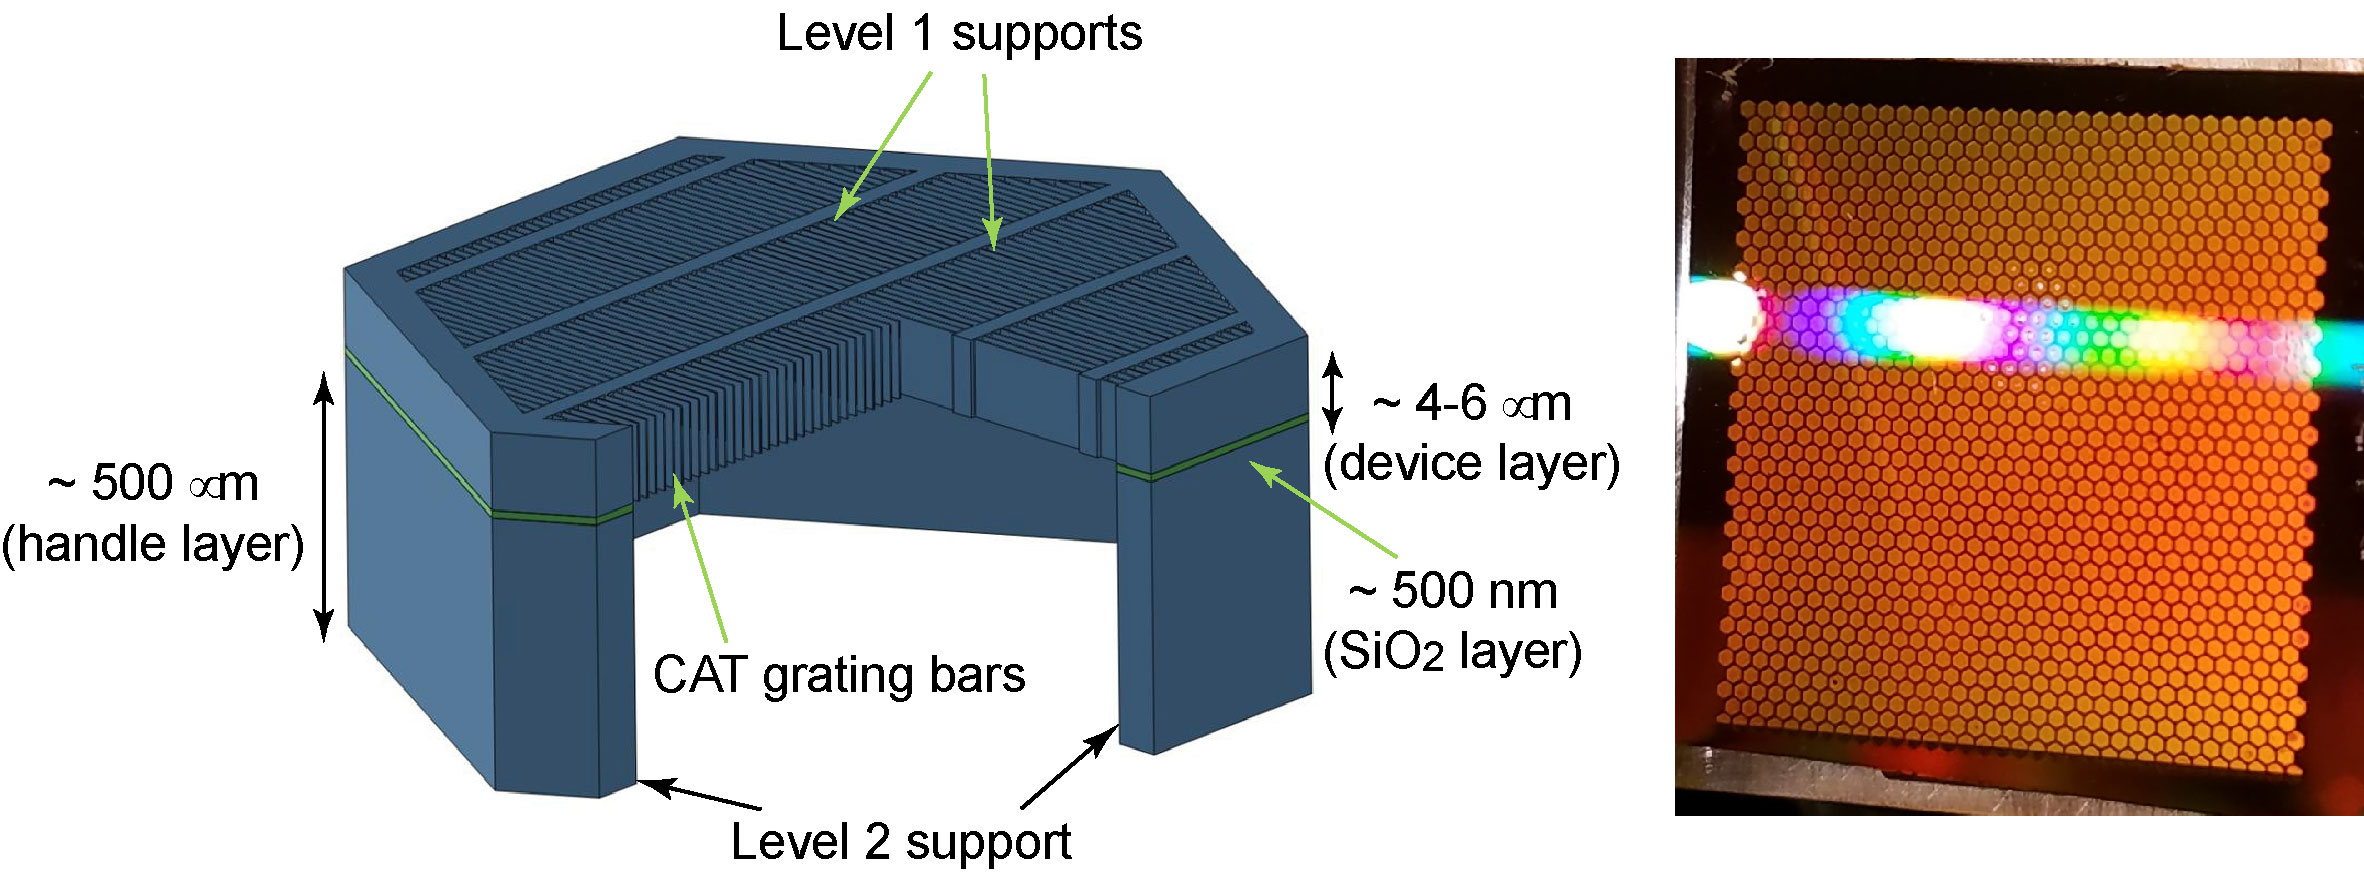
\includegraphics[height=5cm]{unitcell+pic.jpg}
\end{tabular}
\end{center}
\caption {\label{fig:cell}
Left: Schematic depiction of the structural hierarchy of the CAT grating membrane (see text). Right: Photograph of a back-illuminated $32\times32$ mm$^2$ prototype CAT grating membrane, showing the hexagonal L2 mesh and optical diffraction from the L1 mesh.
}
\end{figure}


The XGS is designed with a Rowland torus
geometry\cite{Beuermann:78} where gratings are located on the
Rowland torus. The torus is tilted with respect to the optical axis\cite{doi:10.1117/12.856482,doi:10.1117/12.2273011}, see Figure~\ref{fig:sketch}. That way, gratings with the chosen blaze angle of 1.6~deg are still mostly tangential to the surface of the torus, minimizing the average distance between any point on the flat gratings and the surface of the torus. The torus dimensions are optimized to position the gratings close to the end of the mirror to increase the distance between the focal point and the dispersed signal, as this increases the spectral resolving power $R$.

\begin{figure} [ht]
\begin{center}
\begin{tabular}{c} %% tabular useful for creating an array of images
\includegraphics[width=\textwidth]{rowlandsketch.pdf}
\end{tabular}
\end{center}
\caption {\label{fig:sketch}
Layout of the AXIS/XGS. In both panels, the gray box on the left side indicates the mirror location; its focal point is at the intersection of the horizontal and vertical black lines. The drawing shows a cut through a plane, which contains the symmetry axis of the torus; two blue circles of radius $r$ show the intersection of this plane with the torus and blue dotted lines help to visualize the torus position. For the parameters chosen, the two circles overlap. $\alpha$ is chosen close to the blaze angle to make the blazed grating facets close to tangential to the Rowland Torus. Left: Conceptual sketch; right: to-scale.
}
\end{figure}

\subsection{Filters}

Since X-ray detectors are also sensitive to optical and UV light, we add an optical blocking filter of 30 nm Al topped with 10 nm of aluminum oxide, which may be directly deposited on the detectors. Above that, we simulate a 45~nm layer of Kapton mounted on a 95\% transmissivity metal mesh.


\subsection{Position of detector}
\label{sect:detpos}
\begin{figure} [ht]
\begin{center}
\includegraphics[height=6cm]{detectorplacement.pdf}
\end{center}
\caption {\label{fig:det}
Ray-trace of a continuum source through AXIS/XGS. CAT gratings disperse photons of different energy into different orders, such that most of them end up in a narrow range of angles. The photons distribution has a clear peak at twice the blaze angle, which we call the blaze peak. Detectors only need to cover this narrow region at 400-600~mm distance from the focal point of the mirror to catch the vast majority of photons.
}
\end{figure}
The geometry of CAT gratings favors diffraction orders that direct photons to a specific location (the ``blaze peak'') located 400-600~mm (Figure~\ref{fig:det}) from the focal point, where the detectors for the dispersed spectrum must be placed. The width of this peak depends on wavelength, the depth of the gratings, and the distribution of blaze angle (section~\ref{sect:blaze}) for each grating. To keep the cost and requirements on additional cooling, power, and data volume down, we simulate just 4 CCD-ID94 devices. Those CCDs are rectangular with 2048 times 1024 pixels of 24~$\mu$m size and together cover almost the entire blaze peak. In practice, one might want to use the same detector type that is also mounted in the imaging instrument in the focal plane to simplify integration and testing and later software development and calibration. Detector requirements for the dispersed signal are not very stringent: Since the signal is spread out, count rates are generally lower than in an imaging instrument, thus read-out can be slower and  24~$\mu$m pixels simulated here already oversample the line-spread function and there is no benefit of higher spatial resolution.

Detectors for the dispersed signal are mounted following the Rowland-torus geometry. The imaging detector at the focal point of AXIS, that is planned anyway, can provide information on the zero-order image position for wavelength calibration without placing any additional requirements on that detector.

\subsection{Ray-trace code}
\label{sect:raytrace}

We use the Python-based, open source, Monte-Carlo code MARXS for our ray-trace\cite{marxs1.1,2017AJ....154..243G}. The simulations for this work are run with a development version of MARXS to include AXIS-specific code; that version is publically accessible in the MARXS repository with commit hash: 58b0d43f. Optical properties of materials such as diffraction or transmission probabilities are input from data tables and not calculated by MARXS itself.


\section{Results}
We study different configurations for AXIS and compare the effective area and resolving power. Some of the scenarios use gratings at a high TRL, very similar to what has been demonstrated for Arcus already, while others explore modifications that have not yet been demonstrated to the same level.

\begin{itemize}
  \item The baseline scenario studied here uses $30 * 60$ mm$^2$ flat gratings, where all gratings have exactly the same grating constant. They are arranged such that the short dimension is parallel to the dispersion direction and the long dimension to the cross-dispersion direction. About 1000 gratings are needed to cover the full aperture.
  \item Using larger gratings means that fewer gratings are needed to cover the same geometric area with reduces cost and also losses due to geometric coverage by the grating support structure. A normal Si wafer can yield four $60 * 60$ mm$^2$ gratings, thus these can be manufactured at essentially the same cost per grating as $30 * 60$ mm$^2$ gratings, but only half as many gratings are needed.
  \item When gratings are flat, they deviate from the Rowland torus. This can be compensated by varying the grating period over the grating (``chirp''). Chirped gratings allow us to use huge gratings ($60 * 180$ mm$^2$) without loss of resolving power. Chirped gratings have not yet been demonstrated. In principle, the chirp needed is different for every grating, but in practice, just two or three types of gratings will suffice\cite{10.1117/12.2562878}, keeping complexity and cost down and the total number of gratings is only about 150 to cover the entire aperture.
  \item Alternatively, the gratings can be bend in at least one dimension to follow the Rowland-torus more closely. Laboratory tests of (smaller) bent gratings indicate that the bending does not impact their throughput\cite{10.1117/12.2274205}.
  \item Last, we present simulations where the PSF is dominated by alignment error (the ``round PSF'' scenario described in Sect.~\ref{sect:PSF}). Round is the worst-case for a grating spectrometer, because there is no benefit of subaperturing, but we adjust the in-plane and out-of-plane scatter to keep the total mirror PSF at 1 arcsec HPD. Gratings are arranged as in the baseline scenario.
\end{itemize}


\subsection{A detailed look at the diffraction of 0.6 keV photons}
First, we look at a simulation at one specific energy close to the crucial O~{\sc vii} triplet at 2.1~nm and see how the diffracted orders look on the detector and what we can learn from subaperturing.

Figure~\ref{fig:blaze} shows the distribution of blaze angles for the different scenarios. The position of the detectors is optimized for a specific blaze angle. For flat gratings of finite size, the blaze angle is set for the central ray. That means that photons of a converging beam that pass the grating in a different location will have a different value for the blaze angle. The larger the grating, the larger the range of blaze angles. This leads to broader blaze peak (Fig.~\ref{fig:det}) and photons will be lost unless the read-out detector is expanded. Bending the gratings with a radius of 8.5~m (the average distance of a grating from the focal point) reduces the spread of blaze angles.
\label{sect:blaze}

\begin{figure} [ht]
  \begin{center}
  %\begin{tabular}{c} %% tabular useful for creating an array of images
  \includegraphics[width=0.8\textwidth]{blaze}
  %\end{tabular}
  \end{center}
  \caption {\label{fig:blaze}
    Distribution of blaze angles over all gratings for different grating sizes. For the bent gratings, all photons fall into the same bin, which is cut-off in the figure for display purposes.
  }
\end{figure}

\subsection{Line spread function and subaperturing}
\label{sect:LSF}
We define the resolving power as: $R = \frac{\lambda}{\Delta \lambda} =
\frac{d_x}{FWMH}$ where $\lambda$ is the wavelength of a spectral line with negligible intrinsic width, and $\Delta \lambda$ is the observed width (the ``Line spread function (LSF)'') of this feature. The $FWMH$ is the full width at half maximum of the event distribution, measured in the dispersion direction, and $d_x$ is the distance between the center of a diffracted order and the center of the zeroth order.

\begin{figure} [ht]
\begin{center}
%\begin{tabular}{c} %% tabular useful for creating an array of images
\includegraphics[width=0.8\textwidth]{orders.pdf}
%\end{tabular}
\end{center}
\caption {\label{fig:orders}
  \emph{Left:} Position of gratings in the aperture plane. The gratings are color coded by angle relative to the dispersion direction (positive $y$-axis, here oriented in the horizontal direction).
  \emph{Other panels:} Distribution of photons in the sixth order for different CAT grating sizes and mirror scattering properties for photons of 0.6~keV. Each dot represents a single detected photon, color coded by the grating it passed. Note that the x and y axes are on different scales.
}
\end{figure}

Figure~\ref{fig:orders} shows the distribution of 0.6~keV photons diffracted
into the $6^{\rm th}$ order on the detector for our scenarios.
The left plot in the figure shows the position
of the gratings in the mirror aperture plane. Gratings are colored according to the
\textbf{azimuthal} angle from the dispersion direction. In the other panels, photons are
colored according to the grating they passed through.
The absolute position along the dispersion direction is 53 cm from the focal point, so the dispersion angle is about 4 deg - significantly more than in Chandra or XMM-Newton. Thus, aberations that do not need to be considered for Chandra or XMM-Newton can be important here.

Photons that went through the blue, cyan, and light green colored gratings are distributed narrower than the red points; using only those photons will deliver a lower $FWHM$ and thus higher $R$. We achieve the best spectral resolving power by using only gratings that are located towards the right side of Fig~\ref{fig:orders} (left panel). This differs from typical subaperturing approaches because in-plane and out-of-plane scatter on the mirror surface differ only by a factor of two in our baseline scenario (Sect.~\ref{sect: PSF}) and the dispersed order is located about 53~cm from the optical axis and the facets go from -60~cm (red) to +60~cm (cyan). There is a considerable path length difference between those photons. The light green facets are located directly above the order, while the red/blue ones are 1.5~m to the side.

Figure~\ref{fig:howtosubaperture} shows how much better the spectral resolving power can be for different opening angles of the subaperture. That angle measures the angle between the center of a facet and the positive horizontal axis. For example, a subaperture angle of 30 degrees includes the cyan gratings, 90 deg includes blue over cyan to light green. Only the full aperture (subaperture angle 180 deg) includes all gratings, even the red ones.

\begin{figure} [ht]
  \begin{center}
  %\begin{tabular}{c} %% tabular useful for creating an array of images
  \includegraphics[width=0.4\textwidth]{howtosuabperture.pdf}
  %\end{tabular}
  \end{center}
  \caption {\label{fig:howtosubaperture}
    Distribution of detected photons in the dispersion direction for different subaperture angles. The scaling along the $y$ direction is arbitrary in this figure. The zero point of the $x$-axis is set to be the center of the simulated distribution. This is the same data as in Figure~\ref{fig:orders}, but displayed as a histogram along the cross-dispersion direction.
  }
\end{figure}

For all the scenarios, the photons passing through gratings located close to perpendicular to the dispersion direction (green line) have the sharpest peaks. The other lines differ from the green line in two ways: They are often wider and in some cases their peaks are shifted. The width of the distribution is due to the intrinsic mirror PSF and the fact that the gratings deviate from the Rowland torus. In our simulations, the gratings are placed such that the center of each grating matches the Rowland torus. Because of the tilt of the torus, gratings located in the range $60-90^\circ$ are almost tangential to the torus surface and have the smallest average deviation and thus the sharpest LSF. Larger gratings have larger average deviations than smaller gratings and thus the green LSF in the $60\;\mathrm{mm}\times 30\;\mathrm{mm}$ scenarios is narrower than in the $60\;\mathrm{mm}\times 60\;\mathrm{mm}$ scenario. Gratings located at larger or smaller angles cannot be tangential because they have to be rotated to match the blaze angle specification. Thus, they deviate more from the surface of the torus, leading to wider LSFs (lower $R$). Thus, these simulations show that a higher $R$ can be achieved if only certain parts of the aperture are filled with gratings. As the size of the grating increases, the spots get wider and $R$ is reduced, unless gratings are chirped or bend.

A second effect is the shift in the peak of the LSF between the green line and the other angles' ranges; this is due to the fact that for gratings tangential to the Rowland torus, the average distance of the grating to the detector is larger than for gratings that intersect the Rowland torus. The latter is required in some locations to keep the blaze angle in the specified range.


The two scenarios $60\;\mathrm{mm}\times 30\;\mathrm{mm}$ and $60\;\mathrm{mm}\times 30\;\mathrm{mm}$ (scatter) use the same gratings, but differ in the scatter properties of the mirror. If the mirror PSF is dominated by figure errors and scattering, then subaperturing will increase $R$ a lot more than in the scenario where the PSF is dominated by off-center errors.

\begin{figure} [ht]
  \begin{center}
  \begin{tabular}{c} %% tabular useful for creating an array of images
  \includegraphics[height=6cm]{traderaeff.pdf}
  \end{tabular}
  \end{center}
  \caption {\label{fig:trade}
  Each colored line in this plot is one scenario (grating size, chirp yes/no etc.). The line connects simulations with different subaperturing angle and specific angles are marked with dots (top to bottom filling 100, 83, 67, 50, 33, and 17 \% of the total space with gratings).
  }
\end{figure}

Figure~\ref{fig:trade} shows the trade-off between effective area and $R$. We can choose to populate only part of the aperture with gratings, reducing the effective area and increasing $R$. That choice has to be made based on the science requirements for high-resolution grating spectroscopy.

\subsection{Resolving power and effective area}
To evaluate the resolving power and effective area for a range of photon energies we run ray-traces for the canonical case of $30 * 60$~mm gratings with no bending or chirping. In this early phase of the design, we limit ourselves to a coarse wavelength grid and thus to not resolve all details like chip gaps.

\begin{figure} [ht]
  \begin{center}
  %\begin{tabular}{c} %% tabular useful for creating an array of images
  \includegraphics[width=0.8\textwidth]{RAeff}
  %\end{tabular}
  \end{center}
  \caption {\label{fig:RAeff}
    Effective area (\emph{left}) and resolving power (\emph{right}) for different subaperturing angles.
  }
\end{figure}

Figure~\ref{fig:RAeff} shows the effective area and resolving power $R$. The latter is essentially constant with wavelength, because photons are all diffracted into the blaze peak and for a given spectrograph and mirror, $R$ just depends on the distance between the focal point and the diffracted order.
The effective area of the diffracted signal increases above about 1.2~nm where the Si grating bars reflect the photons. The deep dip around 2~nm is due to one of the two or three relevant orders hitting a chip gap. There should be more chip gaps, but the wavelength resolution of the simulations here is so low that most of them are just stepped over.


\section{Cost}

\textbf{Ed, RANDALL, PETER: Could you write a little bit here?}

\section{Discussion}
We have shown through ray-tracing that AXIS/XGS can reach $R>6000$ with an effective area around 500~cm$^2$ by covering just one third of the aperture with CAT gratings and about three times as much effective area at $R=4000$, if the entire aperture is covered. The CAT gratings simulated here are modest modifications of gratings that have already been manufactured and been aligned and tested in an X-ray beamline\cite{2022arXiv220609013H}. With this design, AXIS/XGS will outperform all existing or accepted future X-ray missions by a wide margin.

Looking at energies of 0.5~keV as an example, the AXIS/XGS with 33\% coverage of the aperture will have about 40 times the effective area and at least 10 times the resolving power of Chandra/LEGTS; it will have two orders or magnitude more effective area than Chandra/HETGS at launch and almost four orders of magnitude more than Chandra/HETGS has today and a factor of 5 better resolving power\cite{2005PASP..117.1144C}; and compared to XMM/RGS our ray-traces show more than one order of magnitude increase in $R$ and about one order of magnitude in effective area.
%The proposed Arcus mission plans for $R$ and effective area 2-3 times lower than what AXIS/XGS can deliver\cite{doi:10.1117/12.2273011}.
Microcalorimaters such as those on XRISM\cite{10.1117/12.2565812} and Athena X-IFU do not reach above $R=200$ at low energies. Such dramatic jump in capability will lead to significant new discoveries in many areas in astrophysics.

Further refinements of the design shown here can be made, but the most important input is to set the science requirements on $R$ and effective area to decide on the subaperturing angle. Options for the CAT gratings with lower TRL include a coating with a metal like Pt which will increase the reflectivity at higher energies and increase the energy range where $R=5000$ is possible to 2~keV, and bending and chirping as simulated above. For the design of the spectrograph, we can optimize the tilt of the Rowland torus or split gratings such that dispersed gratings fall on different channels like the HEG and MEG in Chandra/HETG\cite{2005PASP..117.1144C}: A third of the aperture could be covered with gratings to reach $R>6000$ with an effective area around 500~cm$^2$, while the remaining area could be covered with gratings that diffract in slightly different direction, so that another 1000~cm$^2$ effective area are simultaneously available at a $R>3000$ - still a factor of a few more than any existing instrument.

While not simulated in this work, CAT gratings allow relatively easy tolerances which can be matched by machining alone in many degrees of freedom. Ref~\citenum{10.1117/1.JATIS.5.2.021003} found that $1\sigma$ tolerances are typically several mm for translations and arcminutes or even degrees for rotations. AXIS/XGS has a larger mirror PSF than used in that study, so $R$ will be lower than it would have been for Lynx/XGS\cite{10.1117/1.JATIS.5.2.021003} anyway, and thus requirements for AXIS/XGS would be even looser.


\section{A science example}
AXIS/XGS will deliver a resolving power 5-10 times higher than any instrument ever flown and simultaneously orders of magnitude improvement in effective area compared to the gratings on Chandra and XMM-Newton. Because of the much improved PSF over XMM-Newton, AXIS/XGS can disentangle spectra from moderately crowded fields and obtain many grating spectra at once, when looking at, e.g.\ a stellar cluster.
With this advancement, we can expect ground-breaking results in different fields of astrophysics. Here, we want to just present one example.

\textbf{Dave: Your text here. We can talk about how we do that best. I could generate ARF/RMF pairs, but it's a non-trivial amount of work, so we should decide if that's necessary or if we can do something simpler that is good enough for this purpose.}

% Note add recent SPIE citations for chirp etc.

\section{Summary}


\acknowledgments
Support for this work was provided in part through NASA grant NNX17AG43G and Smithsonian Astrophysical Observatory (SAO)
contract SV3-73016 to MIT for support of the {\em Chandra} X-Ray Center (CXC),
which is operated by SAO for and on behalf of NASA under contract NAS8-03060.
The simulations make use of Astropy, a community-developed core Python package
for Astronomy\cite{2013A&A...558A..33A,astropy}, numpy\cite{numpy}, and
IPython\cite{IPython}. Displays are done with matplotlib\cite{matplotlib}.


\subsection*{Biographies}
\vspace{2ex}\noindent\textbf{Hans Moritz G\"unther} is a research scientist at MIT. He received his undergraduate degree (in 2005) and his PhD (in 2009) in physics from the University of Hamburg, Germany. After that, he worked at the Harvard-Smithsonian Center for Astrophysics and came to MIT in 2015. He is currently the lead developer of MARX, the ray-tracing software used for the Chandra X-ray observatory. His science interests are in star formation using data from the radio to X-rays.

\vspace{1ex}
\vspace{2ex}\noindent\textbf{Ralf K.~Heilmann} is a principal research scientist at the MIT Kavli Institute for Astrophysics and Space Research, and the associate director of the Space Nanotechnology Laboratory (SNL).  He received his Diplom in physics from the FAU Erlangen/N\"urnberg (1991), and his MS (1993) and PhD (1996) in physics from Carnegie Mellon University.  After a postdoc at Harvard he joined the SNL and has since focused on advanced lithography and the development of x-ray optics for astronomy.


% Example for including a video
%\begin{video}
%\begin{center}
%{\includegraphics[height=5cm]{satellite.eps}}
%\\
%\end{center}
%\caption{\label{vid:satellite}This satellite is a still image from Video 1 (Video 1, MPEG, 2.5 MB).}
%\end{video}

\appendix    % this command starts appendixes

%%%%% References %%%%%

\bibliographystyle{spiejour}   % makes bibtex use spiejour.bst
\bibliography{refs2}   % bibliography data in report.bib


%%%%% Biographies of authors %%%%%


\listoffigures
\listoftables

\end{spacing}
\end{document}



\begin{figure} [ht]
\begin{center}
\begin{tabular}{c} %% tabular useful for creating an array of images
\includegraphics[height=7cm]{Lynx_mayavi.png}
\end{tabular}
\end{center}
\caption {\label{fig:mayavi}
Ray-trace simulation of Lynx XGS. The red, green, and blue rectangles are the active area of the CAT gratings. They are arranged on the surface of the Rowland torus. The yellow strip on the right marks the Rowland circle, where the detectors are located (detectors will only be placed on a very small fraction of the yellow strip shown here). Lines show the path of rays through the system. The simulation is monoenergetic. The different colors of the lines indicate into which diffraction order the photons are diffracted. Only photons that pass the gratings and hit the detector are shown, not those that are absorbed by e.g.\ support structures.
}
\end{figure}


\subsection{Effective area and resolving power over the XGS bandpass}

\begin{figure} [ht]
\begin{center}
\begin{tabular}{c} %% tabular useful for creating an array of images
\includegraphics[height=6cm]{aeff_en.pdf}
\includegraphics[height=6cm]{rew_en.pdf}
\end{tabular}
\end{center}
\caption {\label{fig:aeffr}
$A_{\mathrm{eff}}$ and $R$ for different sub-aperturing angles. Drops in $A_{\mathrm{eff}}$ occur when one of the detected orders falls into a chip gap. The $R$ shown is averaged over all detected orders, so if one order is missing, $R$ can show a spike upwards or downwards.
}
\end{figure}
We now present results for a grid of energies assuming perfect alignment.
Figure~\ref{fig:aeffr} shows $A_{\mathrm{eff}}$ and $R$ for different
sub-aperturing. The
$A_{\mathrm{eff}}$ given in the figure is the total effective area summed over all diffraction orders
that are detected on the detector defined in
section~\ref{sect:detpos}. Some chip gaps are visible in the plot of
$A_{\mathrm{eff}}$, but the wavelength grid is too coarse to see all of them. Since more than one order is detected for most wavelengths, the chip
gaps generally lead to a reduced, but still non-zero  $A_{\mathrm{eff}}$ at
that wavelength. A Chandra-like dither pattern could be employed to reduce
their impact. The shown values for $R$ are the efficiency-weighted averages for all detected orders. \textbf{When one order falls into a chip gap, the resolving power can show spikes up or down, when the order missing at that wavelength had a lower or higher than average resolving power.}

\subsection{Usability of the zeroth order}
\label{sect:0order}
\begin{figure} [ht]
\begin{center}
\begin{tabular}{c} %% tabular useful for creating an array of images
\includegraphics[height=6cm]{highen.pdf}
\end{tabular}
\end{center}
\caption {\label{fig:highen}
Fraction of photons removed from the beam if the XGS is inserted. Solid lines are for pure Si gratings, dotted lines are for a scenario with only Pt coated gratings.  Any ratio between the two curves can be chosen, depending on the desired XGS effective area in the $\sim$ 1.5 - 2 keV range. These simulations include shadowing by the gratings frames and support structure. If about two thirds of the aperture are covered with Si gratings, the LXM or HDXI still sees about \textbf{60-70\%} of the flux above 2~keV that it would see without the XGS inserted. Even if all gratings are coated with Pt, that number is still \textbf{more than 30-60\%}.
}
\end{figure}

An important question is how the presence of the gratings interferes with
observations in the zeroth order simultaneous with the dispersed spectra. The position
of the zeroth order is required for wavelength calibration of the diffracted
signal, but especially at energies above 2~keV where $A_{\mathrm{eff}}$ of
the dispersed orders is low, analysis of the zero order microcalorimeter data
becomes important. For example, in young, flaring stars it would be possible to
study the mass accretion in soft X-rays in the diffracted signal and the
hot Fe~K$\alpha$ line in the microcalorimeter simultaneously.
Figure~\ref{fig:highen} shows that the CAT gratings are mostly transparent at high energies. If two-thirds of the aperture are covered with CAT gratings, only \textbf{30-40\%}
of the high-energy photons are absorbed - and these simulations already include
absorption by the mounting structure of the gratings.

\subsection{Calibration tolerances}
\textbf{So far, no science requirement for the absolute wavelength accuracy of the XGS has been specified,\cite{LynxInterimReport} and thus we currently have not studied the calibration of the instrument in detail. Table~\ref{tab:align} gives the alignment requirements for the elements of the Lynx XGS. Once all elements are set at fixed positions, the absolute wavelength scale can be calibrated, e.g.\ by observations of an astronomical emission line source such as Capella. However, the wavelength scale changes if the position of the zeroth-order changes or optical elements move. The position of the zeroth order can be measured in the microcalorimeter, typically with a high signal-to-noise (Sect.~\ref{sect:0order}). In order to achieve an absolute wavelength calibration accuracy of 25~km~s$^{-1}$, the relative change of the location where the dispersed signal is detected compared to the position where it was detected during calibration is then about $10^{-4}$, which corresponds to 0.05~mm. To reach this level, either the focal plane must be temperature controlled to limit thermal expansion, or the relevant temperatures are measured and the change of the XGS camera position with respect to the zeroth order is calibrated for different temperatures. Similarly, this requires that the positions of the gratings are stable. Either a calibration observation is performed each time after the XGS gratings are inserted into the beam or the insertion mechanism has to provide a highly repeatable position.}

